% Chapter Template

\chapter{Sistema de monitoratge} % Main chapter title

\label{SistemaMonitoratge} % Change X to a consecutive number; for referencing this chapter elsewhere, use \ref{ChapterX}

En aquest punt tenim la base necessària per procedir a exposar el treball realitzat des d'un punt de vista de disseny software i implementació dels diferents components. Agafant com a referència la solució proposada al \textit{Capítol 5. Visió general del sistema}, procedirem a desenvolupar els detalls tècnics de cadascun dels components que integren aquest sistema. Començarem per explicar els detalls relacionats amb el disseny i la implementació dels monitors.

\section{Monitors}

Recordem que, dins el nostre context, un \textbf{monitor} consisteix en un \textbf{component software} autònom amb una activitat regular orientada al control de qualitat d'un altre sistema software. Aquest control de qualitat es basa en una col·lecció de dades obtingudes a través d'aquest segon sistema, que ens aporten informació pròpia del context monitorat. Amb aquestes dades, un sistema capacitat per processar i analitzar aquestes dades, es poden generar suggerències de modificacions. Aquesta darrera part, però, queda fora de l'abast del nostre projecte, que centrarà l'activitat dels monitors en la seva tasca principal: la col·lecció de dades sota una sèrie de criteris específics.\\

En general, per tant, volem que el nostre sistema disposi d'un conjunt de monitors heterogenis (i, per tant, de naturalesa i comportament diferents), que puguin ser capaços de gestionar \textbf{processos de monitoratge} de forma paral·lela. És a dir: cadascun d'aquests monitors ha de ser capaç d'inicialitzar processos de monitoratge que s'executin en paral·lel i en segon pla, col·lectin dades d'acord als criteris de cadascun d'aquests processos, i les redireccionin a un tercer component software, encarregat del seu anàlisi.Per tant, necessitem que cadascun d'aquests monitors satisfaci els següents requisits funcionals:

\begin{enumerate}
\item \textbf{Inicialització de procés de monitoratge.} El monitor ha de poder rebre una petició per inicialitzar un nou procés de monitoratge amb una sèrie de paràmetres de configuració que defineixin aquest procés de monitoratge.
\item \textbf{Modificació de procés de monitoratge.} Donat un procés de monitoratge ja existent, el sistema ha de permetre la seva reconfiguració. És a dir: el sistema ha de permetre modificar els paràmetres d'aquest procés i, en conseqüència, alterar el comportament del procés (d'acord amb els criteris que es presenten a continuació.
\item \textbf{Aturada de procés de monitoratge.} Donat un procés de monitoratge ja existent, el sistema ha de permetre la seva aturada. Davant aquesta petició, el procés s'atura, i per tant es deixen de recol·lectar dades sota aquells criteris de monitoratge.
\end{enumerate}

\subsection{Especificacions tècniques}

Tal i com establiem com a objectiu principal del projecte, aquest sistema de monitoratge ha de ser \textbf{heterogeni}. La conseqüència principal d'aquesta característica és que necessitem definir un sistema que contempli que cadascun d'aquests requisits funcionals es garanteixen en la integració dels monitors implementats, i que per tant esdevenen casos d'ús complets i satisfactoris del nostre context. Per fer-ho, i donat que els monitors seran el principal punt de variabilitat del nostre sistema, hem d'afegir un cert nivell d'abstracció, un \textbf{desacoblament} entre els detalls específics de cadascun dels monitors, que ens resulten indiferents per la resta del sistema.\\

Per tant, el primer pas que hem de realitzar és \textbf{dissenyar una arquitectura} i uns \textbf{criteris de configuració genèrics} que satisfacin dos criteris: primerament, que ens permetin integrar tots els monitors implementats sota aquesta proposta al nostre sistema; i en segon lloc, que permetin una independència suficient com per garantir el criteri d'heterogeneïtat dels monitors. Desenvoluparem aquesta proposta analitzant els següents punts:

\begin{enumerate}
\item \textbf{Comportament intern del monitor.} Anàlisi de les necessitats i detalls tècnics del funcionament intern del procés de monitoratge.
\item \textbf{Redirecció de dades col·lectades.} Especificacions tècniques del mètode de gestió i redirecció de dades.
\item \textbf{Configuració dels monitors.} D'acord amb les necessitats anteriors, descriure quins paràmetres necessitarem per configurar els monitors.
\end{enumerate}

\subsubsection{Comportament intern del monitor}

La implementació d'un monitor representa, des d'un punt de vista semàntic, un component software encarregat de monitorar un component software concret. En aquest context específic, entendrem \textbf{monitorar} com la col·lecció periòdica d'un conjunt de dades produïdes de l'execució del sistema software monitorat. En base a aquesta definició, entendrem com a \textbf{procés de monitoratge} el cicle següent:

\begin{enumerate}
\item Inicialització de les estructures de col·lecció de dades
\item Captura de dades durant el transcurs d'un període de temps determinat
\item Enviament de les dades a un tercer component software
\end{enumerate}

Així, de forma periòdica, un procés de monitoratge recull durant un període de temps (o \textbf{\textit{time slot}}) específic totes les dades que el monitor ha estat configurat per recollir. Per tal que els monitors es puguin explotar al màxim, és imprescindible que aquests permetin l'\textbf{execució en paral·lel} de diversos processos de monitoratge, amb possibles diferències en els seus paràmetres de configuració (p.e., aquest \textit{time slot}).\\

Davant aquesta proposta, el comportament i potencial d'un monitor queda molt limitat, ja que elements com p.e. el mètode de recollida de dades, o fins i tot les dades recollides, queden molt limitats. En general, és molt possible que un sistema software pugui ser monitorat mitjançant diferents tècniques, com per exemple l'ús d'APIs, llibreries o components externs, etc. Per aquesta raó, si volem permetre que el nostre monitor ofereixi flexibilitat en aquest aspecte, hem de permetre l'ús de diferents eines, o \textbf{\textit{tools}}, que aquest monitor pot utilitzar indistintament per executar els processos de monitoratge.\\

La integració de diverses \textit{tools} dins un monitor ens permeten no només una variabilitat en l'execució de la col·lecció de dades, sinó també una major fiabilitat i qualitat del monitor com a component software. Ens permet reaccionar, entre d'altres, davant escenaris on l'ús d'un sistema de monitoratge específic deixa de funcionar (p.e. una API que no dona resposta), ja que davant la detecció d'aquest error el canvi de \textit{tool} utilitzada ens permet que el monitor no deixi de ser usable.\\

En resum, necessitem que el monitor sigui capaç de gestionar un nombre indefinit de processos de monitoratge en paral·lel, amb configuracions diferents, i que utilitzin el conjunt de \textit{tools} implementades.

\subsubsection{Redirecció de dades col·lectades}

Un dels objectius de les especificacions tècniques dels monitors és permetre la seva integració, en primer lloc, dins el context del nostre projecte, i en segon lloc, a sistemes tercers que permetin l'anàlisi de les dades recollides durant la seva activitat de monitoratge. D'aquesta manera augmentem el valor propi dels components dissenyats en el projecte, reutilitzable en contexts diferents al plantejat. Per aquesta raó, i per completar l'activitat del monitor, hem de contemplar com dissenyar l'enviament i redirecció de les dades que cada monitor recull i formata durant la seva activitat. \\

Per facilitar aquest aspecte, i permetre també la seva integració dins el sistema general de SUPERSEDE, els monitors integraran la implementació d'enviament de les seves dades a través d'\textbf{Apache Kafka.} Es tracta d'una plataforma distribuïda de \textit{streaming} que ofereix la possibilitat de crear i configurar \textit{pipelines} de dades en temps real que actuen com a canal de comunicació entre diverses aplicacions o components software. L'arquitectura és senzilla: un component software, anomenat \textbf{\textit{producer}}, es comunica amb el servidor Kafka i envia dades de forma periòdica a un \textit{pipeline} específic d'aquest servidor, prèviament configurat i identificament amb el que anomenem Kafka \textit{topic}, un identificador únic d'aquell \textit{pipeline} per aquell desplegament de Kafka. Aquest flux de dades s'encua al servidor, i es redireccionen a uns altres sistemes o aplicacions, anomenats \textbf{\textit{consumers}}, que reben i processen les dades d'un pipeline específic a mesura que es van enviant i processant.\\

En general, l'avantatge principal de Kafka i la justificació del seu ús pel nostre context és que permet una integració còmode i fiable entre diferents aplicacions que necessiten comunicar dades de forma periòdica, garantint la seva arribada. Kafka ofereix una sèrie d'APIs per configurar els \textit{producers} i \textit{consumers}, així com una configuració relativament senzilla del propi servidor. Gràcies a aquestes característiques, podem aprofitar els propis monitors per actuar com a \textit{producers} d'un \textit{stream} de dades, que es correspondrà amb les dades monitorades durant els processos d'execució, i distribuïr-les als diferents \textit{pipelines} o Kafka \textit{topics}. Així, davant possibles ampliacions i expansions d'aquest projecte, podem fàcilment incorporar components d'anàlisi gràcies al desacoblament entre la lògica interna del monitor i l'enviament i captura de dades que l'arquitectura de Kafka ens ofereix.\\

La lògica interna genèrica proposada per la implementació dels monitors serà, per tant, l'ús de l'API de \textit{producer} de Kafka per part dels monitors, pel qual cada procés de monitoratge enviarà de forma periòdica dades a un servidor Kafka específic, o Kafka \textit{endpoint}, i dins aquest desplegament, a un \textit{pipeline} o Kafka \textit{topic} específic.

\subsubsection{Paràmetres de configuració}

Davant les especificacions anteriors, i per garantir el màxim nivell de personalització i configuració dels monitors, cadascun dels processos de monitoratge actius en un monitor ha de permetre definir els paràmetres relacionats amb les possibles variacions i diferències entre aquests processos, tant en temps de creació com durant la seva reconfiguració. En aquest sentit, es proposen els següents paràmetres com a genèrics per a totes les implementacions de monitors:

\begin{itemize}
\item \textbf{\textit{Time slot}}. Expressat en segons, indica la durada de cada període de monitoratge de dades (és a dir, temps que transcorre cada vegada que s'envia un nou \textit{stream} de dades).
\item \textbf{\textit{Tool name}}. Nom de l'eina (\textit{tool}) utilitzada per aquell procés de monitoratge, i que per tant implica la col·lecció d'unes dades específiques utilitzant una tècnica específica.
\item \textbf{\textit{Kafka endpoint}}. Adreça que apunta al servidor on es troba desplegat el sistema Kafka on s'han d'enviar les dades generades, ja sigui \textit{localhost} o URL pública.
\item \textbf{\textit{Kafka topic}}. Identifica el \textit{pipeline} de dades del servidor Kafka on el monitor (\textit{producer} dins el context de Kafka) ha d'enviar les dades.
\end{itemize}

És possible, tal i com veurem més endavant, que alguns monitors requereixin de paràmetres de configuració addicionals, propis del funcionament intern específic del monitor. Per aquest motiu, a banda de proporcionar una configuració bàsica pels monitors amb els paràmetres anteriors, cal permetre també una extensibilitat en quant a paràmetres de configuració.

\subsection{Arquitectura genèrica}

\begin{figure}
\centering
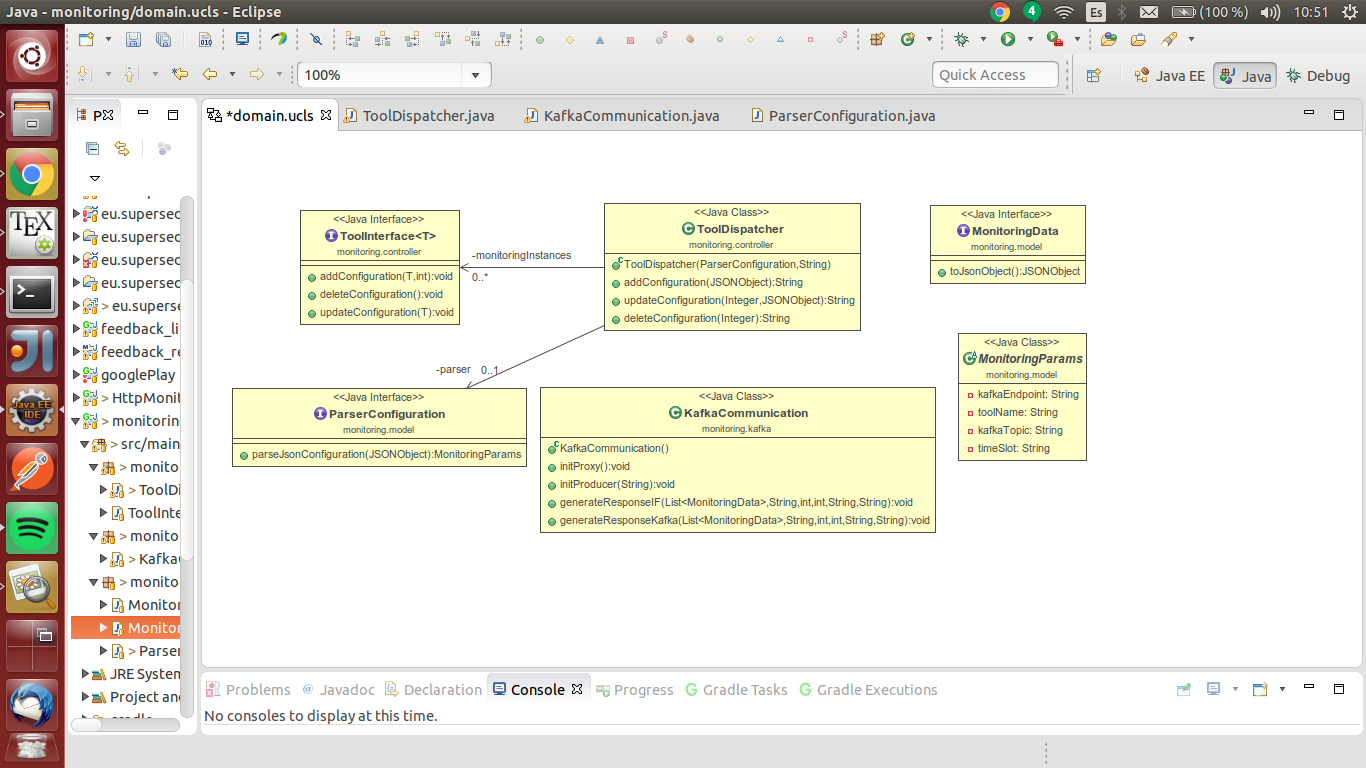
\includegraphics[width=14cm]{Figures/Figure5}
\decoRule
\caption[Arquitectura software genèrica d'un monitor]{Arquitectura software genèrica d'un monitor}
\label{fig:Figura5}
\end{figure}

Es proposa l'arquitectura definida a la Figura 5 a extendre per cadascuna de les implementacions de monitors. Per entendre aquesta arquitectura, a continuació s'expliquen cadascun dels elements integrats:

\begin{itemize}
\item \textbf{MonitoringParams}. Classe abstracta que cada monitor ha d'implementar que conté, de base, els paràmetres de configuració dels monitors genèrics per tots aquests. Addicionalment, cada implementació de monitor pot afegir els paràmetres i la lògica associada a aquests que consideri oportuns.
\item \textbf{ParserConfiguration}. Interfície que cada monitor ha d'implementar i que defineix un mètode per transformar un objecte JSON en una instància de la classe \textit{MonitoringParams} implementada pel propi monitor. L'objectiu és permetre així que el monitor pugui processar JSON com a format de comunicació estàndar per les peticions de configuracions, facilitant el seu ús desplegat com a servei web (especialment útil per l'Integrated Framework dins el context SUPERSEDE, tal i com s'explica al \textit{Capítol 5. Visió general del sistema}).
\item \textbf{ToolInterface}. Interfície parametritzada amb una especialització de la classe \textit{MonitoringParams} que defineix una instància de procés de monitoratge per una \textit{tool} específica. Defineix els següents mètodes:
\begin{itemize}
\item \textbf{\textit{addConfiguration(T)}} -> inicialitza el procés de monitoratge amb els paràmetres definits per la instància de T (subclasse de MonitoringParams)
\item \textbf{\textit{deleteConfiguration()}} -> atura el procés de monitoratge i elimina la instància de la \textit{tool}
\item \textbf{\textit{updateConfiguration(T)}} -> actualitza els paràmetres de configuració del procés iniciat en segon pla per la instància de la \textit{tool}
\end{itemize}
\item \textbf{ToolDispatcher}. Classe que actua com a controlador del monitor, rebent totes les peticions relacionades amb els processos de monitoratge i gestionant les diferents instàncies en execució. Defineix un \textit{ParserConfiguration} per processar la traducció de JSON (format estàndar) a \textit{MonitoringParams} pels següents mètodes:
\begin{itemize}
\item \textbf{\textit{addConfiguration(JSONObject)}} -> processa els paràmetres definits al JSONObject i inicialitza una instància de la \textit{tool} corresponent amb els paràmetres associats
\item \textbf{\textit{deleteConfiguration(int)}} -> atura el procés de monitoratge identificat per l'id proporcionat
\item \textbf{\textit{updateConfiguration(JSONObject, int)}} -> actualitza els paràmetres de configuració definits al JSONObject del procés de monitoratge identificat per int
\end{itemize}
Aquest controlador és perfectament usable per tot monitor implementat d'acord amb la configuració de la resta de classes i interf
\item \textbf{MonitoringData}. Interfície que cada monitor implementa amb les dades i format que el monitor genera fruït de la seva activitat, amb la implementació d'un mètode \textit{toJsonObject()} per definir un format genèric de les dades a enviar
\item \textbf{KafkaCommunication}. Classe que implementa la comunicació amb el servidor de Kafka, i que permet enviar les dades generades per l'activitat de monitoratge. Implementa 4 mètodes segons les dues lògiques de comunicació possibles: la integrada al sistema SUPERSEDE (utilitzant \textit{proxies} de IF), i una configuració personalitzable a un Kafka endpoint específic:
\begin{itemize}
\item \textbf{\textit{initProxy()}} -> inicialitza la instància de \textit{proxy} que permet la comunicació amb el Kafka \textit{server} desplegat a IF
\item \textbf{\textit{generateResponseIF(List<MonitoringData>)}} -> envia el llistat d'instàncies de dades monitorades a través del \textit{proxy} inicialitzat
\item \textbf{\textit{initProducer(String)}} -> inicialitza un \textit{producer} de Kafka que es comunica amb l'\textit{endpoint} especificat
\item \textbf{\textit{generateResponseKafka(List<MonitoringData>)}} -> envia el llistat d'instàncies de dades monitorades a través del \textit{producer} inicialitzat
\end{itemize}
\end{itemize}

Aquesta és per tant la proposta d'una arquitectura genèrica per la implementació de cadascun dels monitors a integrar en el nostre sistema. Les especificacions tècniques tant des d'un punt de vista de requisits funcionals com requisits arquitectònics o de qualitat queden garantides, així com la seva extensibilitat d'acord amb les característiques específiques necessàries de cada monitor. La proposta genèrica s'implementa en un projecte del qual les implementacions de monitors específics han d'extendre com a subprojecte, utilitzant les funcionalitats de Gradle a tal efecte.

\subsection{Implementació de monitors}

Un cop exposada l'arquitectura i especificacions genèriques dels monitors, el següent pas és procedir a la implementació dels diferents monitors que integrarem al nostre sistema. Aquestes implementacions esdevindran possibles casos d'ús a executar, però únicament suposen exemples dins d'un ample ventall de possibilitats d'implementació.

En aquest projecte presentem la implementació de 3 monitors classificats en 2 tipus de monitors diferents: \textbf{monitors de xarxes socials} i \textbf{monitors de botigues d'aplicacions}. Pel primer tipus, es proposa un monitor de la xarxa social \textbf{Twitter}. Pel segon tipus, es proposen dos monitors: un monitor de \textbf{Google Play} i un altre de l'\textbf{App Store}. 

\subsubsection{Twitter Monitor}

L'objectiu d'aquest monitor és supervisar i recol·lectar els tuits publicats a la xarxa social de Twitter durant un període de temps concret (definit al procés de monitoratge) que compleixen una sèrie de característiques específiques, d'acord amb els criteris que poden resultar d'interès en quant a la informació d'aquests tuits. \\

Per permetre aquesta activitat de monitorate, i tal i com procedirem amb cadascun dels monitors, necessitem implementar com a mínim una \textit{tool} amb la qual realitzar el procés de monitoratge. Definirem una \textit{tool} anomenada \textbf{TwitterAPI} que utilitzarà la llibreria \textbf{twitter4j}, una llibreria lliure no oficial de Java que permet utilitzar una arquitectura ja definida per connectar-se a les APIs de Twitter, i entre d'altres a la \textbf{Stream API}, una API que permet obrir \textit{streams} de dades per capturar i processar tots els tuits publicats en temps real que compleixin una sèrie de característiques específiques.\\

Pel nostre cas, definirem dos paràmetres per filtrar els tuits monitorats: l'\textbf{autor} del tuit i l'aparició d'un \textbf{conjunt de paraules} específic al contingut del tuit. Per configurar cadascun dels processos de monitoratge d'acord a aquests dos criteris, caldrà afegir els següents paràmetres:

\begin{itemize}
\item \textbf{accounts} - llistat amb els identificadors dels autors dels quals volem obtenir els tuits 
\item \textbf{keywordExpression} - expressió booleana formada per combinacions AND, OR i NOT de diferents \textit{keywords} que el contingut del tuit ha de satisfer per ser monitorat
\end{itemize}

La \textit{Stream API} ofereix paràmetres de configuració per realitzar el \textit{tracking} dels tuits que satisfan ambdues condicions. En el cas del primer paràmetre \textit{accounts} no cal realitzar cap transformació, ja que únicament necessitem els noms únics de les comptes dels autors per obtenir els seus tuits. Contrariament, l'API únicament ofereix l'oportunitat de filtrar per combinacions de paraules expressades en la seva \textit{forma normal disjuntiva}, o \textbf{FND}. És a dir, expressions del format:\\

\centerline{\textit{$X_{1} \,\, OR \,\, X_{2} \,\, OR \,\, .. \,\, OR \,\, X_{n}$}}\bigskip

\noindent
on $X_{n}$ és una expressió booleana formada per una combinació indefinida d'operands AND:\\

\centerline{\textit{$keyword_{1} \,\, AND \,\, keyword_{2} \,\, AND \,\, .. \,\, AND \,\, keyword_{n}$}}\bigskip

Davant aquest fet, i per evitar forçar un format específic del paràmetre de configuració d'entrada, necessitem implementar una lògica interna pròpia de la \textit{tool} TwitterAPI que transformi qualsevol expressió booleana en la seva expressió FND. 

\subsubsection{Google Play Monitor}

\subsubsection{App Store Monitor}

\section{Monitor Manager}

\section{Orchestrator}
